\documentclass[sigconf,nonacm]{acmart}
\usepackage{amsmath,booktabs,array}
\usepackage{bbm}
\usepackage{tikz}
\usetikzlibrary{arrows.meta,calc,fit,backgrounds}
\definecolor{cblu}{RGB}{50,110,190}\definecolor{cgrn}{RGB}{40,150,70}\definecolor{cora}{RGB}{210,110,30}
\definecolor{cred}{RGB}{200,50,50}\definecolor{cgry}{RGB}{100,100,100}\definecolor{cpur}{RGB}{130,50,170}
\setcopyright{none}
\settopmatter{printacmref=false}
\renewcommand\footnotetextcopyrightpermission[1]{}
\usepackage{enumitem}
\setlist{nosep}
\setlength{\emergencystretch}{3em}
\title{Decision Validity of Security-Twin Remediation: A Research Protocol for Stale Telemetry and Missing Dependencies}
\subtitle{Research protocol, version 0.2, 4 October 2026}
\author{Ezekiel Ologunde}
\affiliation{%
  \institution{Independent Researcher}
  \city{Boston}
  \state{MA}
  \country{USA}}
\email{ologunde@bu.edu}
\renewcommand{\shortauthors}{Ologunde}
\begin{document}
\begin{abstract}
Security twins can predict an acceptable intervention using observations or dependency models that no longer describe the executing system. This protocol proposes a controlled study of that discrepancy in an open microservice application. Observation age, missing dependencies, and approval-to-execution delay will be manipulated while an independent application measurement path evaluates recovery and collateral harm. The candidate contribution is an intervention benchmark and comparative evidence about execution-time revalidation, not the invention of digital twins or abstention. Public telemetry will support input validation; new treatment outcomes will be generated in a reproducible testbed. This document contains hypotheses and proposed methods. No remediation experiment has been run and no effectiveness result is reported.
\end{abstract}
\keywords{digital twins, remediation, stale telemetry, dependency graphs, selective decision-making, research protocol}
\maketitle

\section{Motivation and novelty boundary}
GuardedAct already combines twin simulation, blast-radius prediction and a rollback gate. Its discussion explicitly assumes complete dependency information and acknowledges replay limitations \cite{guarded}. CCSS-IX and DEPLOY-RL already study selective intervention/deployment decisions and conservative risk evaluation \cite{ccss,deploy}. Network-twin work assesses counterfactual effects of configuration changes \cite{sixg}. Therefore neither a confidence gate nor measuring false-safe approvals is itself new.

Our proposed distinction is a controlled joint perturbation study of observation age and missing service edges, followed by revalidation at the execution boundary. This is a provisional empirical contribution. An explicit limitation in a prior paper motivates testing; it does not establish that no other work addresses the limitation. The accompanying dossier records competing approaches and unresolved full-text comparisons. Its review is focused, not systematic.

\section{Questions and falsifiable hypotheses}
\textbf{RQ1:} What are the separate and interacting effects of observation age and random dependency omission on false-safe initial approvals? \textbf{RQ2:} At a fixed 50\% selection fraction, does joint evidence scoring reduce false-safe risk compared with fixed confidence? \textbf{RQ3:} Does fresh execution-time revalidation outperform a frozen-evidence recheck after the same delay? \textbf{RQ4:} How does performance change under withheld workload and dependency patterns? \textbf{RQ5:} What recovery cost accompanies abstention under a fixed fallback policy? RQ1 and RQ2 are confirmatory; RQ3 through RQ5 are exploratory.

\begin{description}[style=nextline]
\item[H1, primary mechanism hypothesis.] Joint corruption increases the probability of a false-safe decision beyond the sum of the isolated increases, on an additive risk scale. For a fixed comparator gate, define $F=\mathbbm{1}\{A=1,V=1\}$, where $A$ means approved and $V$ means independently verified violation. The proposed interaction is
\[
\begin{aligned}I={}&P(F\mid s_1,m_1)-P(F\mid s_1,m_0)\\&-P(F\mid s_0,m_1)+P(F\mid s_0,m_0)>0.\end{aligned}
\]
The primary contrast uses fresh versus two observation periods old and zero versus 20\% randomly omitted edges. Targeted omissions and the full dose-response grid are secondary. A point estimate alone cannot falsify the population hypothesis. An interval spanning zero is inconclusive; an interval entirely at or below zero is incompatible with a positive interaction at the chosen confidence level.
\item[H2, primary selection hypothesis.] At a fixed 50\% selection fraction in a prespecified batch of opportunities, a joint observable-evidence score yields lower false-safe risk than a fixed-confidence score. Models are frozen before test evaluation. Selection uses scores and deterministic outcome-blind tie breaking, never reference outcomes. This tests ranking quality and is not an online deployment policy. Freshness-only and residual-only comparisons are secondary.
\item[Exploratory expectations.] Fresh evidence may improve final authorization relative to a matched-delay frozen-evidence recheck (RQ3); benefit may weaken under shift (RQ4); abstention may delay recovery (RQ5). Estimate these effects and uncertainty without claiming confirmatory guarantees.
\end{description}

The selection fraction and corruption levels are design choices, not literature-derived safety standards. Pilot feasibility may require amendments, which must be recorded before the confirmatory protocol is frozen.

\section{Conceptual framework}
The study combines selective decision-making with controlled causal contrasts. It does not propose a new theory. Assigned age and hidden dependencies may alter model-state mismatch, which influences predicted validity and initial approval. Delay and intervening state changes may invalidate that approval. Revalidation changes final authorization; executed actions and abstention affect both recovery and harm. Workload, service, fault and action are effect modifiers. These relationships are hypotheses, not established causal findings. Conditioning on approval changes case composition, so conditional risk must be accompanied by all-opportunity outcomes. No formal mediation analysis is planned. Figure~\ref{fig:framework} summarizes these proposed relationships and the research question addressed at each stage.

\begin{figure*}[t]
\centering
\resizebox{\textwidth}{!}{%
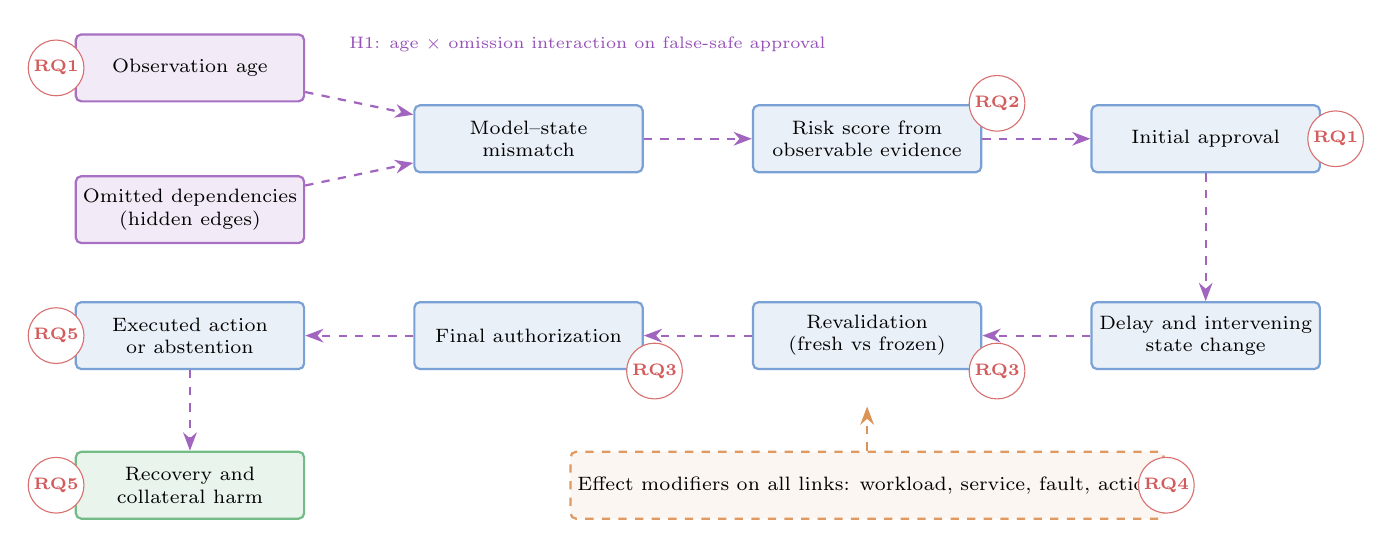
\begin{tikzpicture}[font=\fontsize{6.6pt}{8pt}\selectfont, >=Stealth,
  box/.style={rectangle, rounded corners=2pt, draw=cgry!60, thick, fill=cgry!8, minimum width=2.9cm, minimum height=0.85cm, text centered, align=center, inner sep=2.5pt},
  inp/.style={box, draw=cpur!70, fill=cpur!10},
  dec/.style={box, draw=cblu!65, fill=cblu!10},
  outb/.style={box, draw=cgrn!65, fill=cgrn!10},
  mod/.style={box, draw=cora!70, dashed, fill=cora!6, minimum width=7.2cm},
  hyp/.style={-{Stealth}, thick, cpur!75, dashed},
  tag/.style={circle, draw=cred!70, fill=white, text=cred!80, inner sep=1.2pt, font=\fontsize{5.6pt}{6.8pt}\selectfont\bfseries}]
\node[inp] (age) at (0,1.2) {Observation age};
\node[inp] (om) at (0,-0.6) {Omitted dependencies\\ (hidden edges)};
\node[dec] (mm) at (4.3,0.3) {Model--state\\ mismatch};
\node[dec] (rs) at (8.6,0.3) {Risk score from\\ observable evidence};
\node[dec] (ia) at (12.9,0.3) {Initial approval};
\node[dec] (dl) at (12.9,-2.2) {Delay and intervening\\ state change};
\node[dec] (rv) at (8.6,-2.2) {Revalidation\\ (fresh vs frozen)};
\node[dec] (fa) at (4.3,-2.2) {Final authorization};
\node[dec] (ex) at (0,-2.2) {Executed action\\ or abstention};
\node[outb] (rc) at (0,-4.1) {Recovery and\\ collateral harm};
\node[mod] (md) at (8.6,-4.1) {Effect modifiers on all links: workload, service, fault, action};
\draw[hyp] (age) -- (mm);
\draw[hyp] (om) -- (mm);
\draw[hyp] (mm) -- (rs);
\draw[hyp] (rs) -- (ia);
\draw[hyp] (ia) -- (dl);
\draw[hyp] (dl) -- (rv);
\draw[hyp] (rv) -- (fa);
\draw[hyp] (fa) -- (ex);
\draw[hyp] (ex) -- (rc);
\draw[-{Stealth}, thick, cora!75, dashed] (md.north) -- (8.6,-3.1);
% H1 and RQ tags
\node[font=\fontsize{5.8pt}{7pt}\selectfont, text=cpur!85, anchor=west] at (1.9,1.5) {H1: age $\times$ omission interaction on false-safe approval};
\node[tag] at (-1.7,1.2) {RQ1};
\node[tag] at (14.55,0.3) {RQ1};
\node[tag] at (10.25,0.75) {RQ2};
\node[tag] at (10.25,-2.65) {RQ3};
\node[tag] at (5.9,-2.65) {RQ3};
\node[tag] at (-1.7,-4.1) {RQ5};
\node[tag] at (12.4,-4.1) {RQ4};
\node[tag] at (-1.7,-2.2) {RQ5};
\end{tikzpicture}}
\caption{Conceptual framework. Every dashed link is a proposed relationship, not an established finding. Assigned observation age and hidden dependencies may widen the mismatch between the modeled and executing state, which feeds an observable-evidence risk score and the initial approval; later delay or state change may invalidate that approval; revalidation changes final authorization, which determines executed actions, abstention, recovery and collateral harm. Red tags show the research question addressed at each stage (RQ1 and RQ2 confirmatory; RQ3--RQ5 exploratory). Conditioning on approval changes case composition, so conditional risk is always reported with all-opportunity outcomes. No formal mediation analysis is planned.}
\Description{Flow diagram of proposed, hypothesized relationships. Observation age and omitted dependencies feed model-state mismatch, then a risk score, then initial approval. Initial approval is followed by delay and intervening state change, then revalidation, then final authorization, then executed action or abstention, then recovery and collateral harm. An effect-modifier box for workload, service, fault and action acts on all links. Tags mark which research question applies at each stage.}
\label{fig:framework}
\end{figure*}

\section{Resources and evidence roles}
\begin{table*}[t]
\caption{Resources and their intended evidence roles.}
\label{tab:resources}
\small
\begin{tabular}{>{\raggedright\arraybackslash}p{0.17\textwidth}>{\raggedright\arraybackslash}p{0.38\textwidth}>{\raggedright\arraybackslash}p{0.38\textwidth}}
\toprule Resource & Intended role & Boundary \\
\midrule
DeathStarBench \cite{dsb} & Open executable social-network application; generate new paired intervention outcomes & Independently instrumented software reference, not a real production system. \\
RCAEval \cite{rca} & Public observational failure telemetry; check adapters and sensitivity to diagnosis/measurement features & Diagnosis labels are not counterfactual repair labels. Cross-application transfer must be evaluated, not assumed. \\
MicroRemed \cite{micro} & Inspect existing live remediation evaluation before implementing duplicate infrastructure & No claim of reproducing it until code, licensing and the relevant protocol have been checked. \\
BATADAL \cite{batadal} & Optional future water-network extension & Simulated observations do not establish physical safety or microservice calibration. \\
\bottomrule
\end{tabular}
\end{table*}

The feasibility download contains an RCAEval-linked example CSV with 721 rows and 59 columns, and BATADAL normal-operation data with 8,761 rows and 45 columns. Both passed a basic empty-cell audit. These are schema checks, not scientific findings. Full dataset splits and intervention experiments are pending. Repository revisions and file hashes are retained separately; no external paper PDFs are included in the Overleaf upload.

\section{Experimental system}
\subsection{Reference application and twin}
Deploy the pinned open application in an isolated local Linux container environment. Docker and WSL executables are present on the current Windows host, but runtime readiness and capacity have not been verified. Freeze image digests, resource limits, workload seeds, clock behavior, and observation interval after the pilot. Figure~\ref{fig:system} shows the proposed system and the separation between policy-visible and evaluator-only information.

\begin{figure*}[t]
\centering
\resizebox{\textwidth}{!}{%
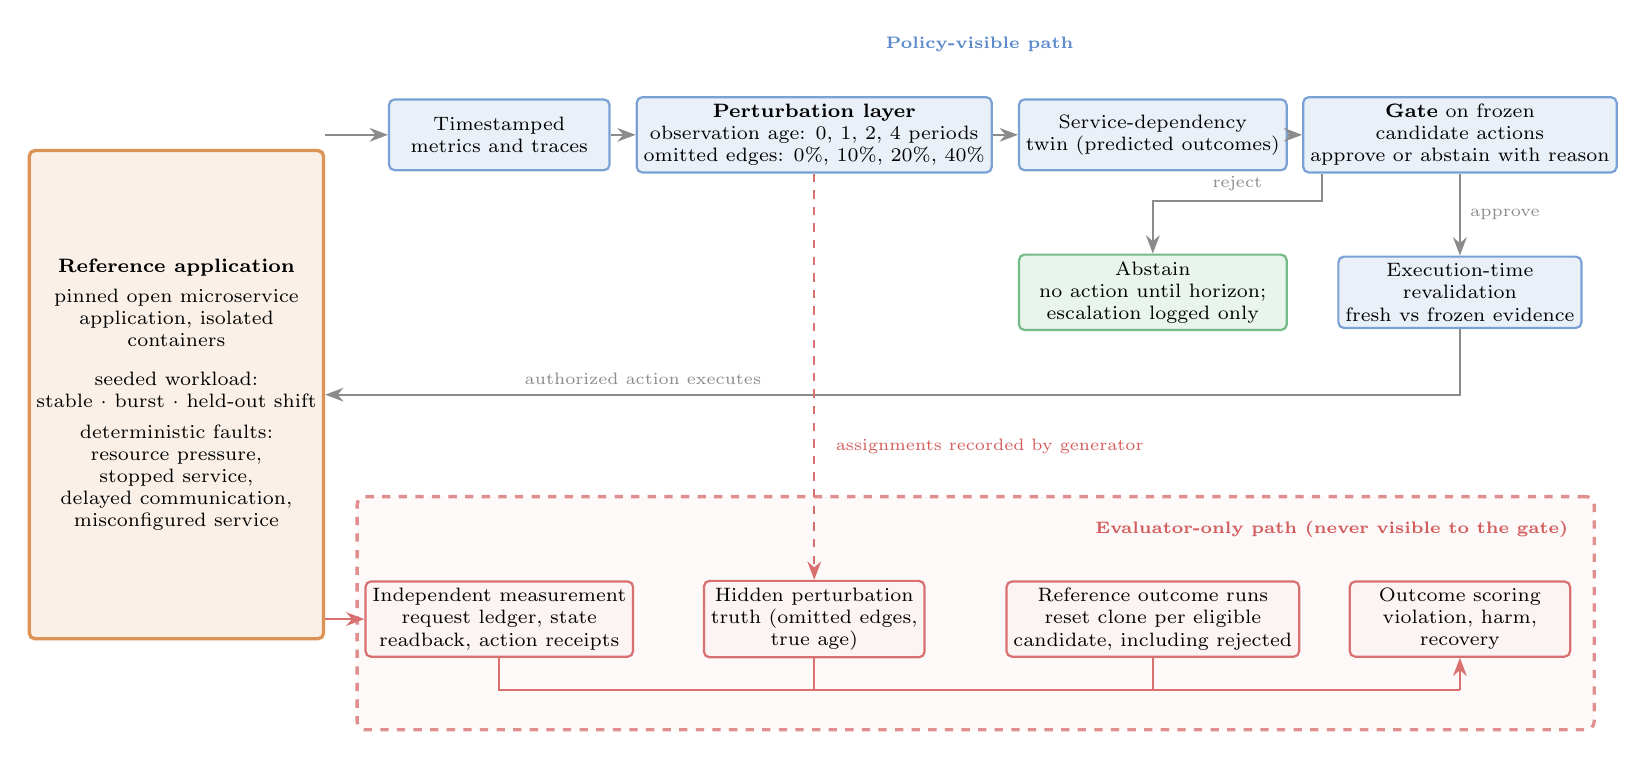
\begin{tikzpicture}[font=\fontsize{6.6pt}{8pt}\selectfont, >=Stealth,
  box/.style={rectangle, rounded corners=2pt, draw=cgry!60, thick, fill=cgry!8, minimum width=2.8cm, minimum height=0.9cm, text centered, align=center, inner sep=2.5pt},
  pol/.style={box, draw=cblu!65, fill=cblu!10},
  app/.style={box, draw=cora!75, very thick, fill=cora!10, minimum width=2.8cm, minimum height=6.2cm},
  evl/.style={box, draw=cred!70, fill=cred!6},
  abst/.style={box, draw=cgrn!65, fill=cgrn!10},
  arr/.style={-{Stealth}, thick, cgry!75}]
\node[app] (app) at (0,0.1) {\textbf{Reference application}\\[3pt] pinned open microservice\\ application, isolated\\ containers\\[6pt] \scriptsize seeded workload:\\ \scriptsize stable $\cdot$ burst $\cdot$ held-out shift\\[3pt] \scriptsize deterministic faults:\\ \scriptsize resource pressure,\\ \scriptsize stopped service,\\ \scriptsize delayed communication,\\ \scriptsize misconfigured service};
\node[pol] (tele) at (4.1,3.4) {Timestamped\\ metrics and traces};
\node[pol, minimum width=3.5cm] (pert) at (8.1,3.4) {\textbf{Perturbation layer}\\ \scriptsize observation age: 0, 1, 2, 4 periods\\ \scriptsize omitted edges: 0\%, 10\%, 20\%, 40\%};
\node[pol] (twin) at (12.4,3.4) {Service-dependency\\ twin (predicted outcomes)};
\node[pol, minimum width=3.0cm] (gate) at (16.3,3.4) {\textbf{Gate} on frozen\\ candidate actions\\ \scriptsize approve or abstain with reason};
\node[pol, minimum width=3.0cm] (rev) at (16.3,1.4) {Execution-time\\ revalidation\\ \scriptsize fresh vs frozen evidence};
\node[abst, minimum width=3.4cm] (abs) at (12.4,1.4) {Abstain\\ \scriptsize no action until horizon;\\ \scriptsize escalation logged only};
\node[font=\fontsize{6pt}{7.4pt}\selectfont\bfseries, text=cblu!80] at (10.2,4.55) {Policy-visible path};
\draw[arr] (app.east |- tele.west) -- (tele.west);
\draw[arr] (tele) -- (pert);
\draw[arr] (pert) -- (twin);
\draw[arr] (twin) -- (gate);
\draw[arr] (gate.south) -- node[right, font=\fontsize{5.6pt}{7pt}\selectfont] {approve} (rev.north);
\draw[arr] (gate.south west) ++(0.25,0) -- ++(0,-0.35) -| node[pos=0.25, above, font=\fontsize{5.6pt}{7pt}\selectfont] {reject} (abs.north);
\draw[arr] (rev.south) -- (16.3,0.1) -- node[pos=0.72, above, font=\fontsize{5.6pt}{7pt}\selectfont] {authorized action executes} (app.east |- 0,0.1);
% evaluator-only region
\begin{scope}[on background layer]
\node[draw=cred!55, dashed, very thick, rounded corners=3pt, fill=cred!3, fit={(2.4,-4.05)(17.9,-1.3)}, inner sep=3pt] (ev) {};
\end{scope}
\node[font=\fontsize{6pt}{7.4pt}\selectfont\bfseries, text=cred!80, anchor=north east] at (17.8,-1.38) {Evaluator-only path (never visible to the gate)};
\node[evl] (led) at (4.1,-2.75) {Independent measurement\\ \scriptsize request ledger, state\\ \scriptsize readback, action receipts};
\node[evl] (tru) at (8.1,-2.75) {Hidden perturbation\\ truth \scriptsize (omitted edges,\\ \scriptsize true age)};
\node[evl, minimum width=3.4cm] (out) at (12.4,-2.75) {Reference outcome runs\\ \scriptsize reset clone per eligible\\ \scriptsize candidate, including rejected};
\node[evl] (sco) at (16.3,-2.75) {Outcome scoring\\ \scriptsize violation, harm,\\ \scriptsize recovery};
\draw[arr, cred!70] (app.east |- led.west) -- (led.west);
\draw[cred!70, thick] (led.south) -- (4.1,-3.65) -- (16.3,-3.65);
\draw[cred!70, thick] (tru.south) -- (8.1,-3.65);
\draw[cred!70, thick] (out.south) -- (12.4,-3.65);
\draw[arr, cred!70] (16.3,-3.65) -- (sco.south);
\draw[arr, dashed, cred!70] (pert.south) -- (tru.north);
\node[font=\fontsize{5.6pt}{7pt}\selectfont, text=cred!80, anchor=west] at (8.25,-0.55) {assignments recorded by generator};
\end{tikzpicture}}
\caption{Experimental system and information separation. The policy-visible path (blue) receives timestamped telemetry after the assigned perturbations (observation age and random edge omission), feeds a service-dependency twin and a gate, and optionally revalidates before executing a typed action on the reference application; an abstention performs no intervention until the fixed horizon. The evaluator-only path (red dashed) records independent outcomes and reference outcomes for every eligible candidate (including rejected ones) in reset clones, and stores the hidden perturbation truth separately. The gate has no access to this path. Twin predictions never serve as reference labels. This is a design diagram of the proposed testbed; the testbed has not been deployed and the figure contains no results.}
\Description{Block diagram. Top row, policy-visible path: telemetry and traces pass through a perturbation layer that sets observation age and omitted edges, into a service-dependency twin and a gate. The gate approves into execution-time revalidation, whose authorized action executes on the reference application, or abstains with no action until the horizon. Bottom row, a dashed evaluator-only region contains independent measurement, reference outcome runs on reset clones, hidden perturbation truth, and outcome scoring, separated from the gate.}
\label{fig:system}
\end{figure*}


Implement the candidate twin as a service-dependency model driven by timestamped metrics and traces. Keep its predicted outcomes and gate logic separate from the reference measurement path. The reference must execute actions on the application and observe externally issued requests, successful writes/reads, latency, errors and recovery. Predictions from the twin must never become the reference labels. Shared instrumentation remains a common-mode risk and should be checked against an independent request ledger.

The declared deployment graph and a prespecified instrumented workload suite define an experimental reference graph. It is not omniscient knowledge of all possible real-world dependencies. Deliberately removed edges are hidden from the decision policy. The policy cannot use the true omission percentage or the evaluator's graph.

\subsection{Scenarios and actions}
Use deterministic fault injection initially: resource pressure, stopped service, delayed communication and a misconfigured service. Add an isolated containment scenario in which blocking a specified communication edge removes an explicitly defined unwanted test flow while legitimate transactions must continue. This uses synthetic traffic and does not require attacks against external systems.

Candidate actions are typed and bounded: restart one service, restore a known configuration, isolate one declared communication relation, or take no action. Recovery actions and security containment actions must be reported separately. Freeze the action list for all comparison methods. Start with a deterministic proposal generator to isolate the gate effect. An LLM generator is an optional later experiment, not necessary for the initial causal question.

For each scenario, clone/reset the same initial state and execute an intervention arm and a no-action arm with matched workload seed. Obtain reference outcomes for every eligible candidate, including those rejected by a gate, using isolated outcome runs invisible to the policy. Freeze proposals before perturbing policy-visible evidence. Randomize run order and verify reset integrity. Nondeterministic scheduling requires repeated runs and paired analysis, not a claim of exact physical counterfactual equivalence.

For RQ3, hold the proposed action, initial opportunity, scheduled execution time and computation budget constant. Compare revalidation on fresh observations with the same computation on frozen observations after the same delay. Both arms begin from the same initial approvals. The main abstention policy performs no intervention until a fixed horizon and logs escalation only. It does not assume a human repairs the system. An alternative automated fallback, if studied, is a separate arm.

\subsection{Factorial perturbations}
Proposed grid:
\begin{itemize}
\item Observation age: 0, 1, 2, and 4 observation periods. Hold all timestamps and collection delays explicitly.
\item Missing edges: 0\%, 10\%, 20\%, and 40\%; evaluate random omissions and separately targeted omissions of critical dependencies.
\item Approval-to-execution delay: 0, 1, and 2 observation periods, with and without a scheduled dependency change.
\item Workload regime: stable, burst, and held-out shifted request mix.
\end{itemize}
The base age-by-omission grid has 16 cells per scenario; targeted deletion and execution delay are distinct experimental factors. Do not silently pool them. Reject impossible edge-count requests and retain the realized count. Normalizing by observation period makes the design portable but does not imply equivalent dynamics across applications. Figure~\ref{fig:grid} shows the base grid and the primary H1 contrast.

\begin{figure}[t]
\centering
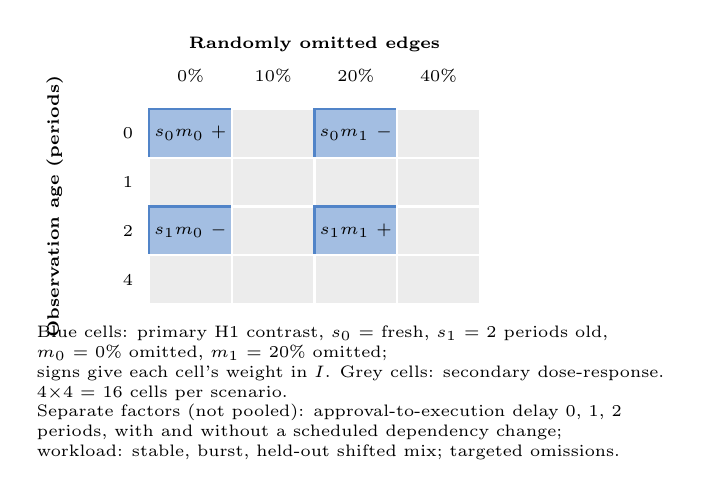
\begin{tikzpicture}[font=\fontsize{6.4pt}{7.8pt}\selectfont]
\node at (2.075,0.42) {0\%};
\node at (3.125,0.42) {10\%};
\node at (4.175,0.42) {20\%};
\node at (5.225,0.42) {40\%};
\node[font=\fontsize{6pt}{7.4pt}\selectfont\bfseries] at (3.650,0.82) {Randomly omitted edges};
\node[anchor=east] at (1.47,-0.310) {0};
\fill[cblu!45, draw=cblu!85, line width=0.8pt] (1.550,-0.620) rectangle (2.600,0.000);
\node at (2.075,-0.310) {$s_0m_0$ $+$};
\fill[cgry!12, draw=white, line width=0.8pt] (2.600,-0.620) rectangle (3.650,0.000);
\fill[cblu!45, draw=cblu!85, line width=0.8pt] (3.650,-0.620) rectangle (4.700,0.000);
\node at (4.175,-0.310) {$s_0m_1$ $-$};
\fill[cgry!12, draw=white, line width=0.8pt] (4.700,-0.620) rectangle (5.750,0.000);
\node[anchor=east] at (1.47,-0.930) {1};
\fill[cgry!12, draw=white, line width=0.8pt] (1.550,-1.240) rectangle (2.600,-0.620);
\fill[cgry!12, draw=white, line width=0.8pt] (2.600,-1.240) rectangle (3.650,-0.620);
\fill[cgry!12, draw=white, line width=0.8pt] (3.650,-1.240) rectangle (4.700,-0.620);
\fill[cgry!12, draw=white, line width=0.8pt] (4.700,-1.240) rectangle (5.750,-0.620);
\node[anchor=east] at (1.47,-1.550) {2};
\fill[cblu!45, draw=cblu!85, line width=0.8pt] (1.550,-1.860) rectangle (2.600,-1.240);
\node at (2.075,-1.550) {$s_1m_0$ $-$};
\fill[cgry!12, draw=white, line width=0.8pt] (2.600,-1.860) rectangle (3.650,-1.240);
\fill[cblu!45, draw=cblu!85, line width=0.8pt] (3.650,-1.860) rectangle (4.700,-1.240);
\node at (4.175,-1.550) {$s_1m_1$ $+$};
\fill[cgry!12, draw=white, line width=0.8pt] (4.700,-1.860) rectangle (5.750,-1.240);
\node[anchor=east] at (1.47,-2.170) {4};
\fill[cgry!12, draw=white, line width=0.8pt] (1.550,-2.480) rectangle (2.600,-1.860);
\fill[cgry!12, draw=white, line width=0.8pt] (2.600,-2.480) rectangle (3.650,-1.860);
\fill[cgry!12, draw=white, line width=0.8pt] (3.650,-2.480) rectangle (4.700,-1.860);
\fill[cgry!12, draw=white, line width=0.8pt] (4.700,-2.480) rectangle (5.750,-1.860);
\node[rotate=90, font=\fontsize{6pt}{7.4pt}\selectfont\bfseries] at (0.35,-1.240) {Observation age (periods)};
\node[align=left, anchor=north west, font=\fontsize{5.9pt}{7.2pt}\selectfont] at (0.0,-2.630) {Blue cells: primary H1 contrast, $s_0$ = fresh, $s_1$ = 2 periods old,\\ $m_0$ = 0\% omitted, $m_1$ = 20\% omitted;\\ signs give each cell's weight in $I$. Grey cells: secondary dose-response.\\ 4$\times$4 = 16 cells per scenario.\\ Separate factors (not pooled): approval-to-execution delay {0, 1, 2}\\ periods, with and without a scheduled dependency change;\\ workload: stable, burst, held-out shifted mix; targeted omissions.};
\end{tikzpicture}
\caption{Base factorial grid per scenario: observation age by randomly omitted edges. The four blue cells are the primary H1 contrast; the interaction is $I=P(F\mid s_1,m_1)-P(F\mid s_1,m_0)-P(F\mid s_0,m_1)+P(F\mid s_0,m_0)$, so the matching-sign cells carry weight $+1$ and the mixed cells weight $-1$. The grid specifies design cells only; it contains no outcome data.}
\Description{A four by four grid. Rows are observation ages of 0, 1, 2 and 4 periods; columns are omitted-edge levels of 0, 10, 20 and 40 percent. Four cells are highlighted: age 0 and 2 crossed with 0 and 20 percent omission. The diagonal pair carries a plus sign and the off-diagonal pair a minus sign in the interaction formula.}
\label{fig:grid}
\end{figure}


\section{Gate and comparison methods}
\begin{enumerate}
\item No selective gate: execute the fixed candidate action, to expose underlying harm.
\item Fixed-confidence twin gate: threshold a calibrated predicted violation score.
\item Freshness-only gate: use observed age with the same candidate actions.
\item Residual-only gate: use recent prediction error without age or dependency evidence.
\item Joint observable-evidence gate: use age, residuals, trace coverage, unseen endpoints, and version changes. Candidate dependency uncertainty sets may be formed from independently sampled trace windows. Their coverage is empirical, not guaranteed.
\item Joint gate with execution-time revalidation: recollect permitted evidence and invalidate approval when versions or evidence bounds change.
\item Evaluator-only complete/fresh-information variant: an unattainable-information ceiling, never a deployable competitor.
\end{enumerate}

Fit simple calibrated logistic risk models before complex alternatives. All fit data, feature selection and thresholds must be separated from test scenarios. An approval requires both predicted recovery and acceptable collateral risk. Otherwise return abstain with a reason. The uncertainty-set variant cannot detect an entirely unobserved edge by magic; this limitation is itself a test case.

These are operationally specified comparison methods inspired by prior work. They must not be labeled exact replications of GuardedAct or CCSS-IX unless their original code and parameterization have actually been reproduced. Include freshness-only revalidation as an ablation if the joint method improves, to separate the value of new evidence from the value of a complex score.

\section{Outcome definitions}\label{sec:outcome}
Let $N$ be all eligible scenario-action opportunities, $A_i$ the initial approval indicator and $V_i$ an independently measured operational violation under that candidate at its scheduled reference execution time. Define
\[
\begin{aligned}\mathrm{FSR}&=\frac{\sum_i A_i V_i}{\sum_i A_i},\qquad \mathrm{Coverage}=\frac{\sum_i A_i}{N},\\
\mathrm{FalseSafeOpportunityRate}&=\frac{\sum_i A_i V_i}{N}.\end{aligned}
\]
If no actions are approved, FSR is undefined, not zero. Report counts, coverage, and uncertainty together. Also report safe rejected opportunities, recovery success, containment success, decision latency, time to recovery and rollback success. Figure~\ref{fig:denom} illustrates the denominators.

\begin{figure}[t]
\centering
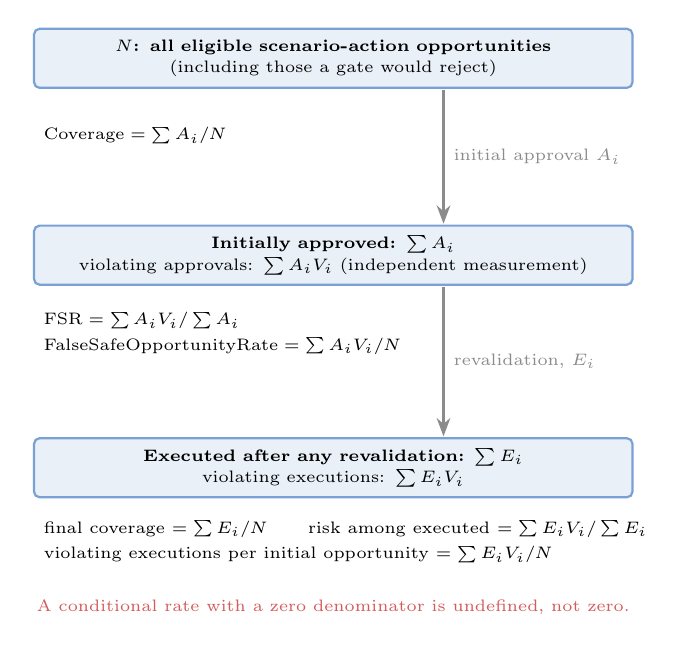
\begin{tikzpicture}[font=\fontsize{6.4pt}{7.8pt}\selectfont, >=Stealth,
  st/.style={rectangle, rounded corners=2pt, draw=cblu!65, thick, fill=cblu!10, minimum width=7.6cm, minimum height=0.75cm, text width=7.3cm, align=center, inner sep=2.5pt},
  arr/.style={-{Stealth}, thick, cgry!75},
  fm/.style={align=left, anchor=north west, font=\fontsize{5.9pt}{7.2pt}\selectfont}]
\node[st] (n) at (0,0) {\textbf{$N$: all eligible scenario-action opportunities}\\ (including those a gate would reject)};
\node[st] (a) at (0,-2.5) {\textbf{Initially approved:} $\sum A_i$\\ violating approvals: $\sum A_iV_i$ (independent measurement)};
\node[st] (e) at (0,-5.2) {\textbf{Executed after any revalidation:} $\sum E_i$\\ violating executions: $\sum E_iV_i$};
\draw[arr] (1.4,-0.4) -- node[right, font=\fontsize{5.8pt}{7pt}\selectfont] {initial approval $A_i$} (1.4,-2.1);
\draw[arr] (1.4,-2.9) -- node[right, font=\fontsize{5.8pt}{7pt}\selectfont] {revalidation, $E_i$} (1.4,-4.8);
\node[fm] at (-3.8,-0.75) {$\mathrm{Coverage}=\sum A_i/N$};
\node[fm] at (-3.8,-3.1) {$\mathrm{FSR}=\sum A_iV_i/\sum A_i$\\[2pt] $\mathrm{FalseSafeOpportunityRate}=\sum A_iV_i/N$};
\node[fm] at (-3.8,-5.75) {final coverage $=\sum E_i/N$\qquad risk among executed $=\sum E_iV_i/\sum E_i$\\[2pt] violating executions per initial opportunity $=\sum E_iV_i/N$};
\node[align=center, anchor=north, font=\fontsize{5.8pt}{7pt}\selectfont, text=cred!80] at (0,-6.75) {A conditional rate with a zero denominator is undefined, not zero.};
\end{tikzpicture}
\caption{Outcome denominators. Initial approval and final execution are distinct stages with distinct denominators, so a revalidation that simply rejects more cannot masquerade as better evidence: conditional risks are always reported beside all-opportunity rates and coverage. Definitions are those of Section~\ref{sec:outcome}.}
\Description{Three stacked boxes joined by downward arrows: all eligible opportunities N; initially approved opportunities, with the subset of violating approvals; and executed opportunities after any revalidation, with the subset of violating executions. Beside each box are the rates defined on it: coverage, false-safe rate, false-safe opportunity rate, final execution coverage, risk among executed, and violating executions per initial opportunity.}
\label{fig:denom}
\end{figure}


Let $E_i$ denote actual execution after any revalidation. Report final execution coverage $\sum E_i/N$, risk among executed actions $\sum E_iV_i/\sum E_i$, and violating executions per initial opportunity $\sum E_iV_i/N$ separately. A zero execution count gives undefined conditional risk. For RQ3, the all-opportunity comparison is primary within the exploratory analysis; differing rejection rates must remain visible. RQ5 reports success by horizon and restricted mean unrecovered time, including abstaining and unrecovered episodes.

Before the main run, freeze transaction-level operational requirements using benign reference runs and an explicit engineering rationale. Initial pilot checks include preservation of acknowledged writes, absence of cross-user data exposure in synthetic accounts, error rate and latency relative to the paired no-action trajectory, and achievement of the action's stated goal within a fixed horizon. Thresholds and observation horizons are not yet validated and must not be called production SLOs.

Separate a requirement violation from action-attributable collateral damage. An already failing system can violate an absolute requirement without the action worsening it. Estimate additional harm from the paired intervention/control contrast. Recovery failure is distinct from collateral harm; do not collapse these into one favorable composite score.

\section{Splits, statistics and sample size}
Partition by entire scenario family and workload seed, not individual telemetry rows. Use development runs to fit the twin, separate calibration runs to set gates, and untouched test runs for evaluation. Withhold at least one service/fault pairing and one dependency-change pattern for transfer analysis. Chronological public-telemetry splits must avoid overlapping windows and train/test preprocessing leakage.

For H2, freeze scores before evaluating test outcomes. Within prespecified scenario strata, choose the lowest-risk half of candidate opportunities with a deterministic outcome-blind tie rule; record the achieved count when a stratum is odd-sized. Use the identical selection count for both methods. This confirmatory batch-ranking comparison is distinct from deployment. For secondary online-policy evaluation, lock calibration-derived thresholds and report actual test coverage without retuning. Never transfer a batch-ranking result into a claim of guaranteed online coverage.

Use paired scenario-level contrasts with cluster bootstrap confidence intervals, clustering all corruption cells and action variants that share a base scenario and seed. Treat telemetry samples as repeated measurements, not independent experiments. Test H1 and H2 as the two confirmatory comparisons, with Holm correction at familywise 0.05; other contrasts are exploratory. Report effect sizes and intervals even when a null is not rejected.

The pilot will estimate event frequency, cluster variability, runtime and feasible coverage. It is excluded from confirmatory inference. Power both the H1 interaction and the H2 risk difference using simulation of independent scenario clusters, targeting at least 80\% power with multiplicity accounted for; use the larger sample requirement. The provisional minimum useful H2 improvement is five percentage points; the H1 minimum useful interaction must be specified before the main run. Freeze the sample size and analysis code before accessing test outcomes. If risk is too low or compute is inadequate, revise the estimand before lock or report an estimation study. No sample size is currently claimed sufficient. Zero observed events do not establish zero risk; avoid reporting an all-zero bootstrap interval as certainty.

Unknown reference outcomes remain unknown. Report their counts and best/worst-case bounds, assigning them nonviolating and violating outcomes in turn. Only infrastructure failures meeting a written pre-run rule may be rerun, with original receipts retained. Maintain a dated amendment log recording what information was already available at each change.

\section{Reproducibility and validity checks}
Each run must store a scenario ID, workload seed, source revision, image digests, graph revision, telemetry timestamps, action proposal, gate outcome/reason, execution receipt, independent outcomes and reset verification. Persist the generator's hidden perturbation truth separately from policy-visible inputs. Release generated synthetic traces and schemas under an explicit license once dependencies permit it.

Required checks include a fresh/full-graph control, a deliberately harmful action control, a no-action control, a failed-reset detector, clock-age checks, and an evaluator-blinding test that confirms the gate cannot access hidden labels. Account for unavailable observations as missing, not healthy zeros. Failed runs and timeouts remain in the accounting with predeclared handling, rather than being silently discarded.

Principal threats are incomplete reference instrumentation, shared simulator/evaluator assumptions, artificial edge removal, testbed-scale workload behavior, action-set bias, calibration shift and selection induced by abstention. No empirical success establishes universal safety, production readiness or physical-process validity.

\section{Execution gates and publication package}
\begin{enumerate}
\item Complete the closest-work comparison, including the executable artifacts of RA-DT and E2E-REME; revise the novelty claim if needed.
\item Deploy and validate the open reference; reproduce stable benign behavior and independent outcomes.
\item Run the feasibility pilot; freeze thresholds, requirements, runtime environment, hypotheses, sample size and exclusions in version 1.0.
\item Run confirmatory and transfer experiments; preserve all outcomes and generate analysis tables/figures from machine-readable records.
\item Write the full manuscript with actual findings, limitations, data/code availability, and appropriate target-journal formatting. Archive reproducibility artifacts and verify a clean Overleaf build.
\end{enumerate}
Current status: literature dossier, proposed protocol and initial public-file audits prepared. Baseline deployment, pilot, hypothesis tests and the final journal manuscript remain outstanding. Null and adverse results will be reported. This package is not a completed research article. Figure~\ref{fig:gates} shows the gate sequence and status.

\begin{figure*}[t]
\centering
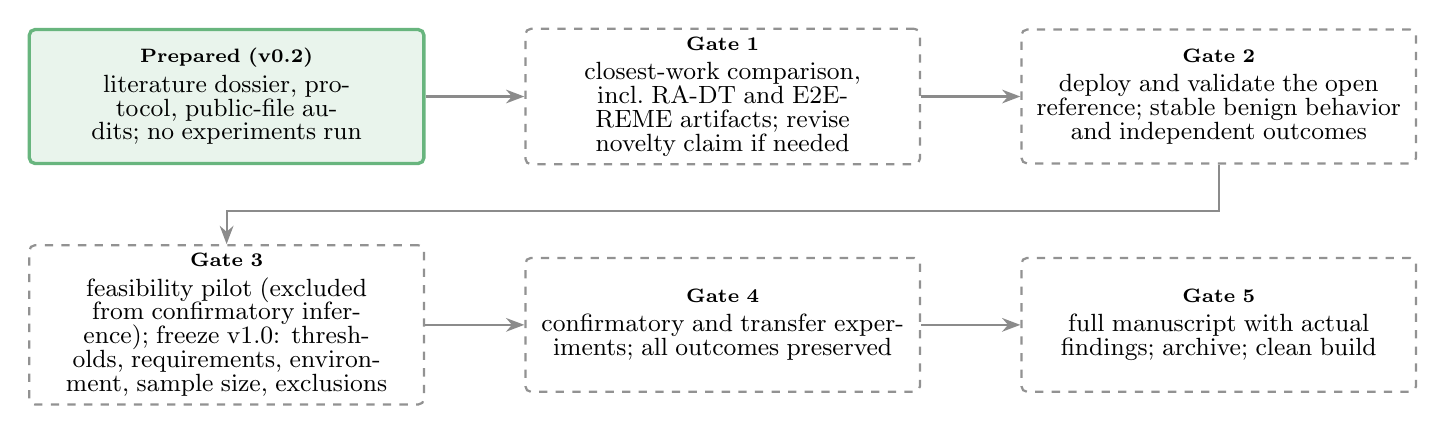
\begin{tikzpicture}[font=\fontsize{7pt}{8.6pt}\selectfont, >=Stealth,
  done/.style={rectangle, rounded corners=2pt, draw=cgrn!70, very thick, fill=cgrn!10, minimum width=5.0cm, minimum height=1.7cm, text width=4.8cm, align=center, inner sep=3pt},
  todo/.style={rectangle, rounded corners=2pt, draw=cgry!70, dashed, thick, fill=white, minimum width=5.0cm, minimum height=1.7cm, text width=4.8cm, align=center, inner sep=3pt},
  arr/.style={-{Stealth}, thick, cgry!75}]
\node[done] (p) at (0,0) {\textbf{Prepared (v0.2)}\\[2pt] \small literature dossier, protocol, public-file audits; no experiments run};
\node[todo] (g1) at (6.3,0) {\textbf{Gate 1}\\[2pt] \small closest-work comparison, incl.\ RA-DT and E2E-REME artifacts; revise novelty claim if needed};
\node[todo] (g2) at (12.6,0) {\textbf{Gate 2}\\[2pt] \small deploy and validate the open reference; stable benign behavior and independent outcomes};
\node[todo] (g3) at (0,-2.9) {\textbf{Gate 3}\\[2pt] \small feasibility pilot (excluded from confirmatory inference); freeze v1.0: thresholds, requirements, environment, sample size, exclusions};
\node[todo] (g4) at (6.3,-2.9) {\textbf{Gate 4}\\[2pt] \small confirmatory and transfer experiments; all outcomes preserved};
\node[todo] (g5) at (12.6,-2.9) {\textbf{Gate 5}\\[2pt] \small full manuscript with actual findings; archive; clean build};
\draw[arr] (p) -- (g1);
\draw[arr] (g1) -- (g2);
\draw[arr] (g2.south) -- (12.6,-1.45) -- (0,-1.45) -- (g3.north);
\draw[arr] (g3) -- (g4);
\draw[arr] (g4) -- (g5);
\end{tikzpicture}
\caption{Execution gates and current status, read left to right and then continuing on the second row. Solid green marks work already prepared; dashed boxes are outstanding. The study cannot proceed past a gate without completing the preceding one; confirmatory testing begins only after the version 1.0 freeze.}
\Description{Sequence of six boxes in two rows of three. The first, solid, is the prepared version 0.2 package. Five dashed boxes follow in order: closest-work comparison, reference deployment and validation, feasibility pilot and freeze of version 1.0, confirmatory and transfer experiments, and the full manuscript with archive. An elbow arrow links the end of the first row to the start of the second.}
\label{fig:gates}
\end{figure*}


\begin{thebibliography}{99}
\bibitem{guarded} W. Cai et al. \emph{Can AI Remediate Backend Failures Safely? GuardedAct with Blast-Radius-Aware Sandboxing}. Preprint, 2026. \url{https://arxiv.org/abs/2609.11264}.
\bibitem{ccss} G. Simethy, D. Ortiz Arroyo, and P. Durdevic. \emph{Explainable Wastewater Digital Twins: Adaptive Context-Conditioned Structured Simulators with Self-Falsifying Decision Support}. Preprint, 2026. \url{https://arxiv.org/abs/2605.19826}.
\bibitem{deploy} Y. Jang et al. \emph{DEPLOY-RL: Active Boundary Discovery and Conservative Certification for Deployable Reinforcement Learning in Safety-Critical Continuous Processes}. IJCAI, 2026. \url{https://www.ijcai.org/proceedings/2026/0718.pdf}.
\bibitem{sixg} J. Jimenez Agudelo et al. \emph{Towards Trustworthy 6G Network Digital Twins: A Framework for Validating Counterfactual What-If Analysis in Edge Computing Resources}. Preprint, 2026. \url{https://arxiv.org/abs/2604.14787}.
\bibitem{dsb} DeathStarBench maintainers. \emph{Open-source benchmark suite for cloud microservices}. Repository, inspected 4 October 2026. \url{https://github.com/delimitrou/DeathStarBench}.
\bibitem{rca} L. Pham et al. \emph{RCAEval: A Benchmark for Root Cause Analysis of Microservice Systems with Telemetry Data}. 2024, revised 2025. \url{https://arxiv.org/abs/2412.17015}. Dataset: \url{https://huggingface.co/datasets/phamquiluan/RCAEval}.
\bibitem{micro} \emph{MicroRemed: Benchmarking LLMs in Microservices Remediation}. Preprint, 2025. \url{https://arxiv.org/abs/2511.01166}. Repository: \url{https://github.com/LLM4AIOps/MicroRemed}.
\bibitem{batadal} R. Taormina et al. \emph{The Battle of the Attack Detection Algorithms: Disclosing Cyber Attacks on Water Distribution Networks}. Journal of Water Resources Planning and Management, 144(8), 2018. \url{https://doi.org/10.1061/(ASCE)WR.1943-5452.0000969}. Data: \url{https://www.batadal.net/data.html}.
\end{thebibliography}
\end{document}
